%----------------------------------------------------------------------------------------
% DE POISSONVERDELING. Alle opgaven zijn eigen werk.
%
% Opbouw: Probleem, Start, leerstof (theorie, werkwijze of uitleg, voorbeeld, korte oefening), en op een
% nieuwe pagina de Opdrachten (door elkaar, stijgende moeilijkheid), Koppel en Test jezelf.
% Labels van dit hoofdstuk beginnen met h2-. De hoogtes van de staven zijn met Python berekend.
%----------------------------------------------------------------------------------------

\mychapter{2}{De Poissonverdeling}

\begin{probleem}
\naast{De spoedafdeling van een klein ziekenhuis houdt elke nacht een aantal bedden vrij voor patiënten die moeten blijven. Uit de gegevens van de voorbije jaren blijkt dat er per nacht gemiddeld 2,4 zulke patiënten binnenkomen, maar het ene moment is het rustig en het andere stroomt het binnen. Elk vrijgehouden bed kost geld, en een patiënt zonder bed moet naar een ander ziekenhuis. Hoeveel bedden moet de afdeling vrijhouden, zodat ze er in minstens 95~\% van de nachten genoeg heeft?}{\begin{tikzpicture}[x=1cm,y=1cm,font=\scriptsize]
  \foreach \i in {0,1,2}{\foreach \j in {0,1}{%
    \begin{scope}[shift={(\i*1.25,\j*1.05)}]
      \draw[accent,thick,fill=accent!10,rounded corners=1pt] (0,0) rectangle (1,.42);
      \draw[accent,thick,fill=white,rounded corners=2pt] (.06,.24) rectangle (.34,.38);
      \draw[accent,thick] (0,0) -- (0,-.14) (1,0) -- (1,-.14);
    \end{scope}}}
  \node[text=accent,font=\Large\bfseries] at (1.75,2.3) {?};
  \fill[fel!80!black] (3.3,2.35) circle (.3); \fill[white] (3.43,2.45) circle (.26);
\end{tikzpicture}}
\end{probleem}

\lkr{Leerplan Complementair (III-WiCo-d): LPD 48 (discrete verdelingen gebruiken om kansen te bepalen), het deel over de Poissonverdeling uit de wenk. Voorkennis uit pakket 4: de binomiale verdeling met verwachtingswaarde en variantie (Kansrekenen, hoofdstuk 3 en 4), het getal $\e$ als limiet van $(1 + \frac1n)^n$ en de afgeleide van $\ln x$ (Exponentiële en logaritmische functies, Limieten en afgeleiden). De som van de kansen, de verwachtingswaarde en de variantie steunen op de reeks $\e^x = \sum \frac{x^k}{k!}$ uit de cursus Reeksen (hoofdstuk 3). Reeksen is zelf een module van Complementair: wie ze niet zag, aanvaardt de reeks en controleert met het rekentoestel dat de partieelsommen naar $\e^x$ gaan (oefening \ref{oef:h2-start-1}f en de Koppel). De vergelijking van waargenomen en verwachte aantallen in 2.3 is een opstap naar de chi-kwadraattoets van hoofdstuk 4. Op de TI-84: \texttt{poissonpdf($\lambda$,k)} en \texttt{poissoncdf($\lambda$,k)} in het menu DISTR.}

Hoeveel mensen bellen in het komende uur naar een hulplijn? Hoeveel drukfouten staan er op een bladzijde, hoeveel rozijnen zitten er in een broodje, hoeveel deeltjes registreert een geigerteller in tien seconden? Telkens tel je hoe vaak iets gebeurt in een stuk tijd of ruimte, en er is geen vast aantal pogingen zoals bij de binomiale verdeling: er kunnen 0, 1, 2 of meer voorvallen zijn, zonder duidelijke bovengrens. Toch volgen zulke aantallen bijna altijd hetzelfde patroon. In dit hoofdstuk leid je dat patroon af uit de binomiale verdeling, de Poissonverdeling, en leer je wanneer het een goed model is. Op het einde weet je hoeveel bedden de spoedafdeling nodig heeft.

\begin{oefeningen}[Start]
\oef{h2-start-1}

\oef{h2-verken}
\end{oefeningen}

\lkr{Laat oefening \ref{oef:h2-verken} maken vóór de uitleg, met het rekentoestel. Leerlingen zien dat de binomiale kansen bijna niet meer veranderen als je het uur in steeds kleinere stukjes verdeelt, en dat de getallen in vraag c al opduiken. Zo is de stelling in 2.1 een antwoord op een vraag die ze zelf gesteld hebben.}

%========================================================================================
\section{Van binomiaal naar Poisson}

\subsection{Een nacht in stukjes}

Waarom is het aantal patiënten in een nacht niet binomiaal? Er is geen vast aantal pogingen: elke inwoner van de streek kan in principe binnenkomen, maar we weten niet hoeveel mensen er die nacht ziek worden of een ongeval hebben. We kennen alleen het gemiddelde, $\lambda = 2{,}4$.

Het idee: verdeel de nacht van 8 uur in $n$ even lange stukjes. Zijn de stukjes kort genoeg, dan komt er in één stukje hoogstens één patiënt binnen, met een kleine kans $p$. De stukjes zijn onafhankelijk van elkaar, en gemiddeld zijn er $np = 2{,}4$ patiënten, dus $p = \frac{2{,}4}{n}$. Het aantal patiënten is dan binomiaal verdeeld, $B\bigl(n, \frac{2{,}4}{n}\bigr)$. Maar welke $n$ kies je? De tabel toont dat het voor grote $n$ niet meer uitmaakt: de kansen naderen een vaste waarde.

\begin{center}
\renewcommand{\arraystretch}{1.3}
\begin{tabular}{|c|c|c|c|c|c|}
\hline
$n$ & 8 \ (per uur) & 80 & 800 & 8000 & $\to +\infty$ \\ \hline
$P(X = 0)$ & 0,0576 & 0,0874 & 0,0904 & 0,0907 & 0,0907 \\ \hline
$P(X = 2)$ & 0,2965 & 0,2643 & 0,2616 & 0,2613 & 0,2613 \\ \hline
\end{tabular}
\end{center}

Ook de staafdiagrammen tonen het: $B(8;\, 0{,}3)$, $B(40;\, 0{,}06)$ en de limiet hebben allemaal gemiddelde 2,4, en verschillen steeds minder.

\figuren{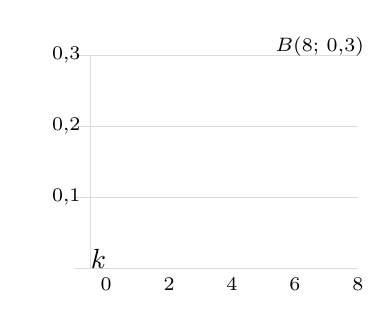
\begin{tikzpicture}[x=.4cm,y=9cm,font=\scriptsize]
  \draw[black!14,very thin] (-.5,0) grid[xstep=20,ystep=.1] (8.5,.3);
  \foreach \k/\h in {0/.0576,1/.1977,2/.2965,3/.2541,4/.1361,5/.0467,6/.01,7/.0012,8/.0001}{\staaf{\k}{\h}{.6}}
  \kansassen{-.5}{9}{.33}{$k$}
  \foreach \k in {0,2,...,8}{\node[below] at (\k,0) {\k};}
  \foreach \t/\l in {.1/{0,1},.2/{0,2},.3/{0,3}}{\node[left] at (-.5,\t) {\l};}
  \node[anchor=north east] at (8.5,.34) {$B(8;\, 0{,}3)$};
\end{tikzpicture}\quad
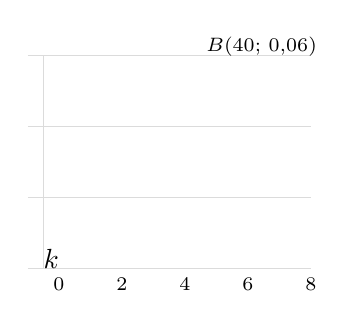
\begin{tikzpicture}[x=.4cm,y=9cm,font=\scriptsize]
  \draw[black!14,very thin] (-.5,0) grid[xstep=20,ystep=.1] (8.5,.3);
  \foreach \k/\h in {0/.0842,1/.2149,2/.2675,3/.2162,4/.1277,5/.0587,6/.0218,7/.0068,8/.0018}{\staaf{\k}{\h}{.6}}
  \kansassen{-.5}{9}{.33}{$k$}
  \foreach \k in {0,2,...,8}{\node[below] at (\k,0) {\k};}
  \node[anchor=north east] at (8.5,.34) {$B(40;\, 0{,}06)$};
\end{tikzpicture}\quad
\begin{tikzpicture}[x=.4cm,y=9cm,font=\scriptsize]
  \draw[black!14,very thin] (-.5,0) grid[xstep=20,ystep=.1] (8.5,.3);
  \foreach \k/\h in {0/.0907,1/.2177,2/.2613,3/.209,4/.1254,5/.0602,6/.0241,7/.0083,8/.0025}{\staaffel{\k}{\h}{.6}}
  \kansassen{-.5}{9}{.33}{$k$}
  \foreach \k in {0,2,...,8}{\node[below] at (\k,0) {\k};}
  \node[anchor=north east] at (8.5,.34) {limiet};
\end{tikzpicture}}

Welke getallen zijn dat? Om de limiet te berekenen, hebben we een limiet nodig die op die van het getal $\e$ lijkt.

\needspace{18\baselineskip}
\subsection{Een limiet voor $\e^x$}

Je kent $\e$ als de limiet van $\bigl(1 + \frac1n\bigr)^n$. In de binomiale kans staat straks $\bigl(1 - \frac{2{,}4}{n}\bigr)^n$: een ander getal dan 1 in de teller, en een minteken. Ook die limiet bestaat.

\begin{theorie}
\begin{stelling}{Limiet voor $\e^x$}
Voor elk reëel getal $x$ is \quad $\formule{\lim_{n \to +\infty} \Bigl(1 + \frac{x}{n}\Bigr)^n = \e^x}$
\end{stelling}

\begin{bewijs}
Voor $x = 0$ staat er $1 = 1$. Neem $x \neq 0$ en $n > |x|$, zodat $1 + \frac{x}{n} > 0$. Dan is
\bewijsregel{\Bigl(1 + \frac{x}{n}\Bigr)^n = \e^{\,n \ln(1 + \frac{x}{n})} .}
Stel $h = \frac{x}{n}$. Als $n \to +\infty$, dan $h \to 0$, en met $n = \frac{x}{h}$ en $\ln 1 = 0$ is
\bewijsregel{n \ln\Bigl(1 + \frac{x}{n}\Bigr) = x \cdot \frac{\ln(1 + h) - \ln 1}{h} \ \to\ x \cdot \ln'(1) = x \cdot \frac11 = x ,}
want de breuk is een differentiequotiënt van $\ln$ in 1. Omdat de exponentiële functie continu is, gaat $\e^{\,n\ln(1 + \frac{x}{n})}$ naar $\e^x$.
\end{bewijs}
\end{theorie}

Met $x = 1$ vind je de bekende limiet voor $\e$ terug. De stelling zegt dat een groei van $x$ die je in $n$ kleine stapjes verdeelt, voor grote $n$ een factor $\e^x$ oplevert. Met $x = -2{,}4$ is $\bigl(1 - \frac{2{,}4}{n}\bigr)^n \to \e^{-2{,}4} \approx 0{,}0907$: precies de kans $P(X = 0)$ uit de tabel.

\voorbeeld{}{Bereken $\displaystyle\lim_{n \to +\infty} \Bigl(1 - \frac{1}{2n}\Bigr)^{n}$.\label{vb:h2-limiet}}{%
\uitleg{De vorm lijkt op die van de stelling, maar in de noemer staat $2n$ en niet $n$. We schrijven de breuk zo dat er $n$ in de noemer staat.}
\begin{stappen}
1 - \frac{1}{2n} = 1 + \frac{-\frac12}{n} & De teller is $x = -\frac12$. \\[2ex]
\lim_{n \to +\infty} \Bigl(1 + \frac{-\frac12}{n}\Bigr)^{n} = \e^{-\frac12} \approx 0{,}607 & De stelling met $x = -\frac12$.
\end{stappen}}

\begin{oefeningen}
\oef{h2-limiet}
\end{oefeningen}

\needspace{18\baselineskip}
\subsection{De limiet van de binomiale kans}

Nu kunnen we de getallen uit de tabel verklaren. We laten $n$ groeien en houden het gemiddelde $np = \lambda$ vast.

\begin{theorie}
\begin{stelling}{Van binomiaal naar Poisson}
Neem $\lambda > 0$ en $k \in \N$. Als $X_n \sim B\bigl(n, \frac{\lambda}{n}\bigr)$, dan is \quad $\formule{\lim_{n \to +\infty} P(X_n = k) = \e^{-\lambda} \frac{\lambda^k}{k!}}$
\end{stelling}

\begin{bewijs}
Neem $n > k$ en $n > \lambda$. We schrijven de binomiale kans zo dat we elke factor apart kunnen bekijken:
\bewijsregel{P(X_n = k) = \binom{n}{k}\Bigl(\frac{\lambda}{n}\Bigr)^k\Bigl(1 - \frac{\lambda}{n}\Bigr)^{n - k} = \frac{n(n - 1) \cdots (n - k + 1)}{k!} \cdot \frac{\lambda^k}{n^k} \cdot \Bigl(1 - \frac{\lambda}{n}\Bigr)^{n - k}}
en dus, door de factoren te herschikken,
\bewijsregel{P(X_n = k) = \frac{\lambda^k}{k!} \cdot \frac{n(n - 1) \cdots (n - k + 1)}{n^k} \cdot \Bigl(1 - \frac{\lambda}{n}\Bigr)^{n} \cdot \Bigl(1 - \frac{\lambda}{n}\Bigr)^{-k} .}
De tweede factor is een product van $k$ breuken, $\frac{n}{n} \cdot \frac{n - 1}{n} \cdots \frac{n - k + 1}{n} = 1 \cdot \bigl(1 - \frac1n\bigr) \cdots \bigl(1 - \frac{k - 1}{n}\bigr)$, en elk gaat naar 1. Ook $\bigl(1 - \frac{\lambda}{n}\bigr)^{-k} \to 1^{-k} = 1$, want $k$ ligt vast. De derde factor gaat naar $\e^{-\lambda}$, volgens de stelling hierboven met $x = -\lambda$. Dus
\bewijsregel{\lim_{n \to +\infty} P(X_n = k) = \frac{\lambda^k}{k!} \cdot 1 \cdot \e^{-\lambda} \cdot 1 = \e^{-\lambda}\frac{\lambda^k}{k!} .}
\end{bewijs}
\end{theorie}

Wat betekenen de factoren van de limiet? Voor grote $n$ is $\binom{n}{k} \approx \frac{n^k}{k!}$: er zijn ongeveer zoveel manieren om de $k$ stukjes met een voorval te kiezen, elk met kans $\bigl(\frac{\lambda}{n}\bigr)^k$. Samen geeft dat $\frac{\lambda^k}{k!}$, waaruit $n$ verdwenen is. De factor $\e^{-\lambda}$ is de limiet van de kans dat er in alle andere stukjes niets gebeurt. Voor $\lambda = 2{,}4$ en $k = 2$ vind je $\e^{-2{,}4} \cdot \frac{2{,}4^2}{2} \approx 0{,}2613$, het getal uit de tabel.

%========================================================================================
\section{De Poissonverdeling}

\subsection{Definitie}

De limiet hangt alleen nog van $\lambda$ af, niet meer van de stukjes. Ze krijgt de naam van de Franse wiskundige Siméon Denis Poisson, die ze in 1837 beschreef in een boek over de kansen bij rechtszaken.

\begin{theorie}
Een toevalsvariabele $X$ met waarden $0, 1, 2, \ldots$ heeft een \textbf{\textcolor{accent}{Poissonverdeling}} met parameter $\lambda > 0$ als

\vspace{1mm}
\qquad $\formule{P(X = k) = \e^{-\lambda}\frac{\lambda^k}{k!}}$ \quad voor $k = 0, 1, 2, \ldots$

\vspace{1mm}
Je schrijft $\formule{X \sim \Poi(\lambda)}$.

\begin{stelling}{Som van de kansen}
Voor $X \sim \Poi(\lambda)$ is \quad $\formule{\sominf{k=0} P(X = k) = 1}$
\end{stelling}

\begin{bewijs}
De Maclaurinreeks van $\e^x$ convergeert voor elke $x$, met som $\e^x$. Met $x = \lambda$ is
\bewijsregel{\sominf{k=0} \e^{-\lambda}\frac{\lambda^k}{k!} = \e^{-\lambda} \sominf{k=0} \frac{\lambda^k}{k!} = \e^{-\lambda} \cdot \e^{\lambda} = 1 .}
\end{bewijs}
\end{theorie}

Een Poissonvariabele heeft oneindig veel mogelijke waarden. Dat is geen probleem: de kansen worden zo snel klein dat een grote waarde praktisch nooit voorkomt. Bij $\lambda = 2{,}4$ is de kans op 10 of meer patiënten in één nacht kleiner dan $0{,}0001$. De som van de kansen is dan een reeks, en die is 1, zoals het hoort. Hoe de verdeling eruitziet, hangt van $\lambda$ af: bij een kleine $\lambda$ is 0 het vaakst, bij een grotere schuift de top naar rechts en wordt de verdeling breder en symmetrischer.

\figuren{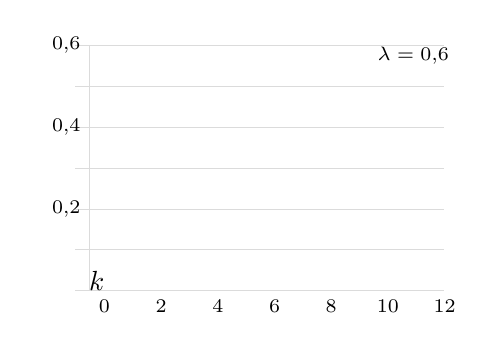
\begin{tikzpicture}[x=.36cm,y=5.2cm,font=\scriptsize]
  \draw[black!14,very thin] (-.5,0) grid[xstep=20,ystep=.1] (12.5,.6);
  \foreach \k/\h in {0/.5488,1/.3293,2/.0988,3/.0198,4/.003,5/.0004}{\staaf{\k}{\h}{.6}}
  \kansassen{-.5}{13}{.64}{$k$}
  \foreach \k in {0,2,...,12}{\node[below] at (\k,0) {\k};}
  \foreach \t/\l in {.2/{0,2},.4/{0,4},.6/{0,6}}{\node[left] at (-.5,\t) {\l};}
  \node[anchor=north east] at (12.5,.62) {$\lambda = 0{,}6$};
\end{tikzpicture}\quad
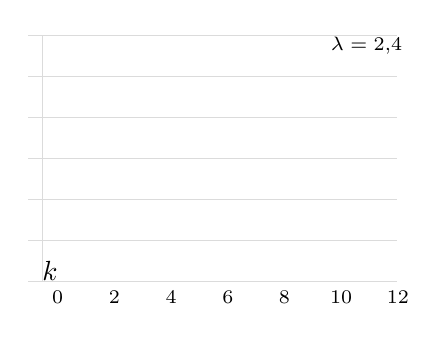
\begin{tikzpicture}[x=.36cm,y=5.2cm,font=\scriptsize]
  \draw[black!14,very thin] (-.5,0) grid[xstep=20,ystep=.1] (12.5,.6);
  \foreach \k/\h in {0/.0907,1/.2177,2/.2613,3/.209,4/.1254,5/.0602,6/.0241,7/.0083,8/.0025,9/.0007}{\staaf{\k}{\h}{.6}}
  \kansassen{-.5}{13}{.64}{$k$}
  \foreach \k in {0,2,...,12}{\node[below] at (\k,0) {\k};}
  \node[anchor=north east] at (12.5,.62) {$\lambda = 2{,}4$};
\end{tikzpicture}\quad
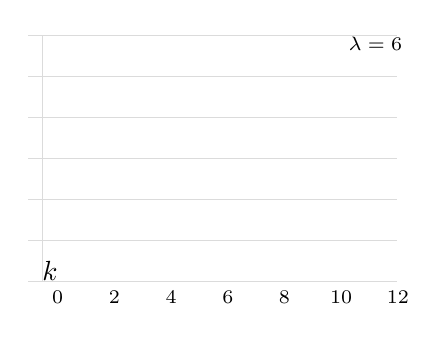
\begin{tikzpicture}[x=.36cm,y=5.2cm,font=\scriptsize]
  \draw[black!14,very thin] (-.5,0) grid[xstep=20,ystep=.1] (12.5,.6);
  \foreach \k/\h in {0/.0025,1/.0149,2/.0446,3/.0892,4/.1339,5/.1606,6/.1606,7/.1377,8/.1033,9/.0688,10/.0413,11/.0225,12/.0113}{\staaf{\k}{\h}{.6}}
  \kansassen{-.5}{13}{.64}{$k$}
  \foreach \k in {0,2,...,12}{\node[below] at (\k,0) {\k};}
  \node[anchor=north east] at (12.5,.62) {$\lambda = 6$};
\end{tikzpicture}}

\voorbeeld{}{Op een drukke kruising gebeuren gemiddeld 1,5 ongevallen per maand. Neem aan dat het aantal ongevallen in een maand Poissonverdeeld is. Wat is de kans op een maand zonder ongeval? En op precies 2 ongevallen?\label{vb:h2-formule}}{%
\uitleg{Het gemiddelde per maand is de parameter: $X \sim \Poi(1{,}5)$. We vullen de formule in met $k = 0$ en $k = 2$.}
\begin{stappenbreed}
P(X = 0) = \e^{-1{,}5} \cdot \frac{1{,}5^0}{0!} = \e^{-1{,}5} \approx 0{,}2231 & Met $1{,}5^0 = 1$ en $0! = 1$. \\[2ex]
P(X = 2) = \e^{-1{,}5} \cdot \frac{1{,}5^2}{2!} \approx 0{,}2510 & Op het rekentoestel: \texttt{poissonpdf(1.5,2)}.
\end{stappenbreed}
In ongeveer 22~\% van de maanden gebeurt er geen ongeval.}

\nujij{Een webshop krijgt gemiddeld 4 bestellingen per uur. Wat is de kans op precies 4 bestellingen in een uur?}{$\e^{-4} \cdot \frac{4^4}{4!} = \e^{-4} \cdot \frac{256}{24} \approx 0{,}195$.}

\begin{oefeningen}
\oef{h2-formule}
\end{oefeningen}

\needspace{16\baselineskip}
\subsection{Cumulatieve kansen}

Vraag je naar \textit{hoogstens} of \textit{minstens}, dan tel je Poissonkansen op, net als bij de binomiale verdeling. Het rekentoestel geeft $P(X \leqslant k)$ meteen met \texttt{poissoncdf($\lambda$,k)}. \textit{Minstens} berekenen we altijd met het complement: er zijn oneindig veel waarden boven $k$, maar maar eindig veel eronder.

\voorbeeld{}{Bij de kruising van het vorige voorbeeld: wat is de kans op hoogstens 2 ongevallen in een maand? Op minstens 3? En op 2, 3 of 4?\label{vb:h2-cumulatief}}{%
\uitleg{\textit{Hoogstens 2} is een cumulatieve kans. \textit{Minstens 3} is er het complement van. Voor de kans tussen twee grenzen trekken we twee cumulatieve kansen af.}
\begin{stappenbreed}
P(X \leqslant 2) = \e^{-1{,}5}\Bigl(1 + 1{,}5 + \frac{1{,}5^2}{2}\Bigr) \approx 0{,}8088 & Drie termen, of \texttt{poissoncdf(1.5,2)}. \\[2ex]
P(X \geqslant 3) = 1 - P(X \leqslant 2) \approx 0{,}1912 & Het complement. \\[1ex]
P(2 \leqslant X \leqslant 4) = P(X \leqslant 4) - P(X \leqslant 1) \approx 0{,}9814 - 0{,}5578 = 0{,}4236 & Van \textit{hoogstens 4} trekken we \textit{hoogstens 1} af, zodat 2 erbij blijft.
\end{stappenbreed}}

\begin{werkwijze}
Bepaal $\lambda$: het gemiddelde aantal voorvallen in het gevraagde interval. Voor $P(X = k)$: de formule of \texttt{poissonpdf($\lambda$,k)}. Voor $P(X \leqslant k)$: \texttt{poissoncdf($\lambda$,k)}. Voor $P(X \geqslant k)$: $1 - P(X \leqslant k - 1)$. Voor $P(k \leqslant X \leqslant m)$: $P(X \leqslant m) - P(X \leqslant k - 1)$.
\end{werkwijze}

\begin{oefeningen}
\oef{h2-cumul}
\end{oefeningen}

%========================================================================================
\section{Verwachtingswaarde en variantie}

\subsection{De formules}

Bij de binomiale verdeling $B\bigl(n, \frac{\lambda}{n}\bigr)$ is het gemiddelde $\lambda$ en de variantie $n \cdot \frac{\lambda}{n}\bigl(1 - \frac{\lambda}{n}\bigr) = \lambda\bigl(1 - \frac{\lambda}{n}\bigr)$. Als $n$ groeit, gaat die variantie naar $\lambda$. Je verwacht dus dat een Poissonverdeling gemiddelde $\lambda$ en variantie $\lambda$ heeft. Dat klopt, maar we bewijzen het rechtstreeks. Omdat $X$ oneindig veel waarden heeft, is de verwachtingswaarde nu een reeks: $\E(X) = \sominf{k=0} k \, P(X = k)$, en ook de rekenformule $\Var(X) = \E(X^2) - \mu^2$ blijft gelden.

\begin{theorie}
\begin{stelling}{Verwachtingswaarde van de Poissonverdeling}
Voor $X \sim \Poi(\lambda)$ is \quad $\formule{\E(X) = \lambda}$
\end{stelling}

\begin{bewijs}
De term met $k = 0$ is nul. Voor $k \geqslant 1$ is $\frac{k}{k!} = \frac{1}{(k - 1)!}$, dus
\bewijsregel{\E(X) = \sominf{k=1} k \, \e^{-\lambda}\frac{\lambda^k}{k!} = \lambda \e^{-\lambda} \sominf{k=1} \frac{\lambda^{k-1}}{(k - 1)!} = \lambda \e^{-\lambda} \sominf{j=0} \frac{\lambda^{j}}{j!} = \lambda \e^{-\lambda} \cdot \e^{\lambda} = \lambda ,}
waarbij we $j = k - 1$ stelden.
\end{bewijs}

\begin{stelling}{Variantie van de Poissonverdeling}
Voor $X \sim \Poi(\lambda)$ is \quad $\formule{\Var(X) = \lambda}$ \quad en \quad $\formule{\sigma = \sqrt{\lambda}}$
\end{stelling}

\begin{bewijs}
Bereken eerst het gemiddelde van $X(X - 1)$. De termen met $k = 0$ en $k = 1$ zijn nul, en voor $k \geqslant 2$ is $\frac{k(k - 1)}{k!} = \frac{1}{(k - 2)!}$. Met $j = k - 2$ is
\bewijsregel{\sominf{k=2} k(k - 1)\, \e^{-\lambda}\frac{\lambda^k}{k!} = \lambda^2 \e^{-\lambda} \sominf{j=0} \frac{\lambda^{j}}{j!} = \lambda^2 .}
Omdat $k^2 = k(k - 1) + k$, is $\E(X^2) = \lambda^2 + \lambda$, de som van twee convergente reeksen. De rekenformule voor de variantie geeft
\bewijsregel{\Var(X) = \E(X^2) - \bigl(\E(X)\bigr)^2 = \lambda^2 + \lambda - \lambda^2 = \lambda .}
\end{bewijs}
\end{theorie}

Bij een Poissonverdeling zijn het gemiddelde en de variantie dus \textit{hetzelfde getal}. Dat is een handige toets voor het model: tel je in een reeks waarnemingen de voorvallen, en ligt de variantie van de aantallen ver van hun gemiddelde, dan is het Poissonmodel waarschijnlijk niet goed. De standaardafwijking $\sqrt{\lambda}$ groeit trager dan $\lambda$: bij een groot gemiddelde schommelen de aantallen relatief minder.

\voorbeeld{}{Een webshop krijgt gemiddeld 3 bestellingen per uur, Poissonverdeeld. Bereken $\mu$ en $\sigma$. Is een uur met 7 of meer bestellingen verrassend?\label{vb:h2-mu}}{%
\uitleg{We gebruiken de formules, en kijken of 7 ver buiten $\mu \pm 2\sigma$ ligt. Daarna berekenen we de kans op 7 of meer, zoals bij de binomiale verdeling.}
\begin{stappenbreed}
\mu = 3, \quad \sigma = \sqrt{3} \approx 1{,}73 & De parameter is zowel gemiddelde als variantie. \\[1ex]
\mu + 2\sigma \approx 6{,}46 & 7 ligt net boven $\mu + 2\sigma$. \\[1ex]
P(X \geqslant 7) = 1 - P(X \leqslant 6) \approx 0{,}0335 & Met \texttt{poissoncdf(3,6)}.
\end{stappenbreed}
In ongeveer 3~\% van de uren: zeldzaam, maar het gebeurt een paar keer per maand.}

\begin{oefeningen}
\oef{h2-mu}
\end{oefeningen}

\needspace{14\baselineskip}
\subsection{Past het model bij de data?}

Kun je aan echte gegevens zien of een Poissonmodel kan kloppen? Een eerste controle is het verband tussen gemiddelde en variantie.

\voorbeeld{}{Twee klantendiensten tellen 50 uur lang het aantal oproepen per uur. Bij de eerste zijn het gemiddelde en de variantie van de 50 aantallen 4,1 en 4,3. Bij de tweede zijn ze 4,1 en 9,8. Bij welke dienst kan een Poissonmodel kloppen?\label{vb:h2-data}}{%
\uitleg{Bij een Poissonverdeling zijn gemiddelde en variantie gelijk. Bij een steekproef van 50 uur zijn ze nooit precies gelijk, maar ze moeten in de buurt liggen.}
\begin{stappenbreed}
\text{dienst 1: } 4{,}1 \approx 4{,}3 & Gemiddelde en variantie liggen dicht bij elkaar: een Poissonmodel met $\lambda \approx 4{,}1$ kan passen. \\[1ex]
\text{dienst 2: } 9{,}8 \text{ is veel groter dan } 4{,}1 & De aantallen schommelen meer dan bij Poisson: geen goed model.
\end{stappenbreed}
Een verklaring voor de tweede dienst: de oproepen zijn niet onafhankelijk. Bij een storing bellen veel klanten tegelijk, en in rustige uren bijna niemand.}

\begin{oefeningen}
\oef{h2-data}
\end{oefeningen}

%========================================================================================
\section{De Poissonverdeling als model}

\subsection{Voorvallen in de tijd of in de ruimte}

Wanneer mag je een Poissonverdeling gebruiken? In 2.1 verdeelden we de nacht in kleine stukjes. Dat werkte omdat de patiënten één voor één binnenkomen, onafhankelijk van elkaar, en omdat het tempo de hele nacht hetzelfde is. De figuur toont zo'n nacht: de tijdstippen liggen willekeurig, soms dicht bij elkaar en soms ver uit elkaar.

\figuren{\begin{tikzpicture}[x=1.65cm,y=1cm,font=\scriptsize]
  \foreach \u in {0,...,8}{\draw[grijs] (\u,-.08) -- (\u,.08); \node[below] at (\u,-.08) {\pgfmathparse{int(mod(22+\u,24))}\pgfmathresult\,u};}
  \draw[->,grijs] (0,0) -- (8.3,0);
  \foreach \t in {.62,2.15,2.4,5.8,7.05,7.2}{\fill[accent] (\t,.22) circle (2.2pt);}
  \foreach \t in {3.1,4.4}{\fill[black!25] (\t,.22) circle (1.6pt);}
  \node[anchor=west] at (8.35,.22) {6 patiënten};
\end{tikzpicture}}

\vspace{-1mm}
\begin{theorie}
Voorvallen vormen een \textbf{\textcolor{accent}{Poissonproces}} als ze één voor één gebeuren, onafhankelijk van elkaar, met een vast gemiddeld tempo $c$ per tijdseenheid. Het aantal voorvallen in een interval met lengte $t$ is dan Poissonverdeeld met

\vspace{1mm}
\qquad $\formule{\lambda = c \cdot t}$
\end{theorie}

Hetzelfde geldt voor voorvallen in de ruimte, met een oppervlakte of een volume in plaats van een tijd: foutjes in een rol stof, rozijnen in deeg, sterren in een stukje van de hemel. Let telkens op de eenheid: $\lambda$ is het gemiddelde in het interval waarnaar gevraagd wordt. Is het tempo niet constant, zoals het aantal klanten in een winkel over een hele dag, dan geldt het model alleen voor een stuk van de dag waarin het tempo ongeveer constant is.

\voorbeeld{}{Een uitgever rekent op gemiddeld 0,4 drukfouten per bladzijde, Poissonverdeeld. Wat is de kans dat een hoofdstuk van 5 bladzijden geen enkele drukfout bevat?\label{vb:h2-tempo}}{%
\uitleg{De vraag gaat over 5 bladzijden, niet over één. We passen $\lambda$ aan het interval aan.}
\begin{stappen}
\lambda = 0{,}4 \cdot 5 = 2 & Het gemiddelde aantal fouten in 5 bladzijden. \\[1ex]
P(X = 0) = \e^{-2} \approx 0{,}1353 & Ongeveer 14~\%.
\end{stappen}
Wie $\lambda = 0{,}4$ gebruikt, berekent de kans op één foutloze bladzijde, $\e^{-0{,}4} \approx 0{,}67$. Dat is de kans voor één bladzijde, niet voor het hele hoofdstuk. Je vindt wel hetzelfde als $\bigl(\e^{-0{,}4}\bigr)^5 = \e^{-2}$: vijf onafhankelijke foutloze bladzijden.}

\begin{werkwijze}
Ga na of de voorvallen één voor één, onafhankelijk en met een vast tempo gebeuren. Reken het gegeven gemiddelde om naar het gevraagde interval: $\lambda = c \cdot t$. Bereken daarna de kans met de formule of het rekentoestel.
\end{werkwijze}

\begin{oefeningen}
\oef{h2-tempo}

\oef{h2-herken}
\end{oefeningen}

\needspace{16\baselineskip}
\subsection{Een benadering van de binomiale verdeling}

Uit 2.1 volgt ook een praktische regel. Is $n$ groot en $p$ klein, dan lijkt $B(n, p)$ op $B\bigl(n, \frac{\lambda}{n}\bigr)$ met $\lambda = np$, en die lijkt op $\Poi(\lambda)$. De figuur vergelijkt $B(50;\, 0{,}04)$ met $\Poi(2)$: de staven zijn bijna even hoog.

\figuren{\begin{tikzpicture}[x=.9cm,y=10cm,font=\scriptsize]
  \draw[black!14,very thin] (-.5,0) grid[xstep=20,ystep=.1] (8.5,.3);
  \foreach \k/\b/\p in {0/.1299/.1353,1/.2706/.2707,2/.2762/.2707,3/.1842/.1804,4/.0902/.0902,5/.0346/.0361,6/.0108/.012,7/.0028/.0034,8/.0006/.0009}{%
    \fill[accent!55] (\k-.32,0) rectangle (\k-.02,\b); \draw[accent] (\k-.32,0) rectangle (\k-.02,\b);
    \fill[fel!80!black] (\k+.02,0) rectangle (\k+.32,\p);}
  \kansassen{-.5}{9}{.32}{$k$}
  \foreach \k in {0,...,8}{\node[below] at (\k,0) {\k};}
  \foreach \t/\l in {.1/{0,1},.2/{0,2},.3/{0,3}}{\node[left] at (-.5,\t) {\l};}
  \fill[accent!55] (5.6,.27) rectangle (5.85,.29); \node[right] at (5.9,.28) {$B(50;\, 0{,}04)$};
  \fill[fel!80!black] (5.6,.23) rectangle (5.85,.25); \node[right] at (5.9,.24) {$\Poi(2)$};
\end{tikzpicture}}

\begin{theorie}
\begin{stelling}{Poissonbenadering}
Is $n$ groot en $p$ klein, dan is \quad $\formule{B(n, p) \approx \Poi(np)}$
\end{stelling}
\end{theorie}

De stelling is een gevolg van de limiet in 2.1, en heeft dus geen apart bewijs. Als vuistregel is de benadering goed als $n \geqslant 50$ en $p \leqslant 0{,}1$. Je rekentoestel kan ook de binomiale kansen berekenen, dus waarom zou je benaderen? Omdat je soms $n$ niet precies kent, zoals het aantal inwoners dat 's nachts ziek kan worden, en omdat de Poissonformule veel eenvoudiger is dan $\binom{n}{k}p^k(1 - p)^{n - k}$ met een grote $n$.

\voorbeeld{}{Eén persoon op 500 heeft een zeldzame bloedgroep. Op een inzameldag komen 1000 donoren. Wat is de kans dat er minstens 3 met die bloedgroep bij zijn? Bereken het exact en met de Poissonbenadering.\label{vb:h2-benadering}}{%
\uitleg{Het aantal is binomiaal, met $n = 1000$ en $p = 0{,}002$. Omdat $n$ groot is en $p$ klein, mag je benaderen met $\lambda = np = 2$.}
\begin{stappenbreed}
\text{exact: } 1 - P(X \leqslant 2) \approx 0{,}323323 & Met \texttt{binomcdf(1000,0.002,2)}. \\[1ex]
\text{benaderd: } 1 - \e^{-2}\Bigl(1 + 2 + \frac{2^2}{2}\Bigr) = 1 - 5\e^{-2} \approx 0{,}323324 & Met \texttt{poissoncdf(2,2)}: pas in de zesde decimaal een verschil.
\end{stappenbreed}}

\begin{oefeningen}
\oef{h2-benader}
\end{oefeningen}

\needspace{16\baselineskip}
\subsection{Een klassieker: de paardentrappen}

Kloppen Poissonkansen met wat je in werkelijkheid telt? Een beroemd voorbeeld komt van de Russisch-Duitse statisticus Ladislaus von Bortkiewicz. In 1898 bestudeerde hij hoeveel soldaten van het Pruisische leger stierven door de trap van een paard. Hij had de gegevens van 10 legerkorpsen gedurende 20 jaar (1875-1894): 200 \textit{korpsjaren}. Een dodelijke trap was zeldzaam en kwam onverwacht, en elk korps had ongeveer evenveel paarden en ruiters. Dat zijn de voorwaarden voor een Poissonmodel.

\voorbeeld{}{In 109 korpsjaren stierf niemand door een paardentrap, in 65 één soldaat, in 22 twee, in 3 drie en in 1 korpsjaar vier. Bereken het gemiddelde aantal doden per korpsjaar, en vergelijk de waargenomen aantallen met die van een Poissonmodel met dat gemiddelde.\label{vb:h2-bortkiewicz}}{%
\uitleg{We schatten $\lambda$ met het gemiddelde van de data. Daarna berekenen we het verwachte aantal korpsjaren met $k$ doden: 200 keer de Poissonkans.}
\begin{stappenbreed}
\lambda = \frac{0 \cdot 109 + 1 \cdot 65 + 2 \cdot 22 + 3 \cdot 3 + 4 \cdot 1}{200} = \frac{122}{200} = 0{,}61 & Het gemiddelde aantal doden per korpsjaar. \\[2.5ex]
200 \cdot P(X = 0) = 200 \, \e^{-0{,}61} \approx 108{,}7 & Verwacht: 108,7 korpsjaren zonder dode. \\[1ex]
200 \cdot P(X = 1) = 200 \, \e^{-0{,}61} \cdot 0{,}61 \approx 66{,}3 & Zo verder voor $k = 2$, 3 en 4.
\end{stappenbreed}
\naast{\renewcommand{\arraystretch}{1.25}
\begin{tabular}{|c|c|c|c|c|c|}
\hline
$k$ & 0 & 1 & 2 & 3 & 4 \\ \hline
waargenomen & 109 & 65 & 22 & 3 & 1 \\ \hline
verwacht & 108,7 & 66,3 & 20,2 & 4,1 & 0,6 \\ \hline
\end{tabular}

\vspace{2mm}
De verwachte aantallen liggen opvallend dicht bij de waargenomen. Ook de variantie van de 200 aantallen is $\frac{196}{200} - 0{,}61^2 \approx 0{,}61$, gelijk aan het gemiddelde.
}{\begin{tikzpicture}[x=.85cm,y=.022cm,font=\scriptsize]
  \draw[black!14,very thin] (-.5,0) grid[xstep=20,ystep=20] (4.5,120);
  \foreach \k/\w in {0/109,1/65,2/22,3/3,4/1}{\staaf{\k}{\w}{.55}}
  \foreach \k/\v in {0/108.7,1/66.3,2/20.2,3/4.1,4/.6}{\fill[fel!80!black] (\k,\v) circle (2pt);}
  \kansassen{-.5}{4.9}{128}{$k$}
  \foreach \k in {0,...,4}{\node[below] at (\k,0) {\k};}
  \foreach \t in {40,80,120}{\node[left] at (-.5,\t) {\t};}
\end{tikzpicture}}}

Hoe dicht moeten de aantallen bij elkaar liggen om het model te aanvaarden? Kleine verschillen zijn altijd te verwachten, ook als het model perfect klopt. In hoofdstuk 4 leer je met de chi-kwadraattoets meten of de verschillen te groot zijn.

\begin{oefeningen}
\oef{h2-past}
\end{oefeningen}

\needspace{18\baselineskip}
\subsection{Terug naar het probleem}

Nu kunnen we de spoedafdeling raad geven. De patiënten komen één voor één binnen, onafhankelijk van elkaar en met een ongeveer vast tempo, dus het aantal per nacht is Poissonverdeeld met $\lambda = 2{,}4$.

\voorbeeld{}{Terug naar het probleem. Hoeveel bedden moet de spoedafdeling vrijhouden, zodat ze er in minstens 95~\% van de nachten genoeg heeft?\label{vb:h2-terug}}{%
\uitleg{Met $b$ bedden is er genoeg plaats als er hoogstens $b$ patiënten komen. We zoeken dus de kleinste $b$ met $P(X \leqslant b) \geqslant 0{,}95$, en proberen $b = 3, 4, 5, \ldots$ met \texttt{poissoncdf(2.4,b)}.}
\naast{\begin{stappenvrij}{3.4cm}{2.6cm}
P(X \leqslant 3) \approx 0{,}7787 & Te weinig. \\[1ex]
P(X \leqslant 4) \approx 0{,}9041 & Nog onder 0,95. \\[1ex]
P(X \leqslant 5) \approx 0{,}9643 & Voldoende.
\end{stappenvrij}}{\begin{tikzpicture}[x=.48cm,y=9cm,font=\scriptsize]
  \draw[black!14,very thin] (-.5,0) grid[xstep=20,ystep=.1] (9.5,.3);
  \foreach \k/\h in {0/.0907,1/.2177,2/.2613,3/.209,4/.1254,5/.0602}{\staaf{\k}{\h}{.6}}
  \foreach \k/\h in {6/.0241,7/.0083,8/.0025,9/.0007}{\staaffel{\k}{\h}{.6}}
  \kansassen{-.5}{10}{.32}{$k$}
  \foreach \k in {0,...,9}{\node[below] at (\k,0) {\k};}
  \foreach \t/\l in {.1/{0,1},.2/{0,2},.3/{0,3}}{\node[left] at (-.5,\t) {\l};}
  \draw[fel!80!black,->] (7.5,.12) node[above,text=black] {te weinig bedden} -- (6.6,.04);
\end{tikzpicture}}
Met 5 bedden is er in ongeveer 96~\% van de nachten genoeg plaats. Met 4 bedden zou ongeveer één nacht op tien te druk zijn.}

Gemiddeld komen er maar 2,4 patiënten, en toch heb je 5 bedden nodig: het gemiddelde is niet genoeg om te plannen, de spreiding telt mee. In het echt kijkt een ziekenhuis ook naar de dag van de week en het seizoen, want het tempo is niet het hele jaar hetzelfde. Hetzelfde soort berekening gebruiken ook brandweerposten, callcenters en websites om hun capaciteit te bepalen.

%========================================================================================
\opdrachtenkop

\begin{oefeningen}
\needspace{10\baselineskip}
\oef{h2-o1}

\oef{h2-o3}

\needspace{10\baselineskip}
\oef{h2-o2}

\needspace{26\baselineskip}
\oef{h2-o4}

\oef{h2-o6}

\oef{h2-o5}

\needspace{10\baselineskip}
\oef{h2-o7}

\oef{h2-o9}

\oef{h2-o8}

\needspace{12\baselineskip}
\oef{h2-o10}

\oef{h2-o12}

\oef{h2-o11}

\oef{h2-o14}

\oef{h2-o13}

\oef{h2-o16}

\oef{h2-o15}

\oef{h2-o17}

\oef{h2-o18}

\needspace{10\baselineskip}
\oef{h2-o19}

\oef{h2-o21}

\oef{h2-o20}

\oef{h2-o22}

\oef{h2-o23}
\end{oefeningen}

%----------------------------------------------------------------------------------------
% KOPPEL: verbanden met andere leerstof
%----------------------------------------------------------------------------------------
\needspace{20\baselineskip}
\opdrachtsectie{Koppel}

\lkr{De eerste oefening gebruikt de Maclaurinreeks van $\e^x$ uit Reeksen (een module van Complementair), de tweede samengestelde interest uit Exponentiële en logaritmische functies, de derde oneigenlijke integralen en partiële integratie uit Integralen, de vierde afgeleiden.}

\begin{oefeningen}
\oef{h2-koppel-1}

\oef{h2-koppel-2}

\oef{h2-koppel-3}

\oef{h2-koppel-4}
\end{oefeningen}

%----------------------------------------------------------------------------------------
\opdrachtsectie{Test jezelf}

\begin{oefeningen}
\oef{h2-t1}

\oef{h2-t2}

\oef{h2-t3}

\oef{h2-t4}

\oef{h2-t5}

\oef{h2-t6}

\oef{h2-t7}
\end{oefeningen}

\herhaalschema{%
  \fv{oef:h2-t1}{vb:h2-limiet}{oef:h2-limiet}%
  \fv{oef:h2-t2}{vb:h2-formule}{oef:h2-formule}%
  \fv{oef:h2-t3}{vb:h2-cumulatief}{oef:h2-cumul}%
  \fv{oef:h2-t4}{vb:h2-tempo}{oef:h2-tempo}%
  \fv{oef:h2-t5}{vb:h2-mu}{oef:h2-mu}%
  \fv{oef:h2-t6}{vb:h2-benadering}{oef:h2-benader}%
  \fv{oef:h2-t7}{vb:h2-terug}{oef:h2-o13}}

\ifzelfstudie
\section*{Maak je eigen samenvatting}
Sluit dit boek en schrijf in je schrift: de limiet van $(1 + \frac{x}{n})^n$ en waarom ze klopt, hoe je de Poissonverdeling uit de binomiale verdeling krijgt, de formule voor $P(X = k)$, waarom de kansen samen 1 zijn, de verwachtingswaarde en de variantie met hun bewijs, de voorwaarden van een Poissonproces en de formule $\lambda = c \cdot t$, wanneer je een binomiale verdeling met Poisson mag benaderen, en hoe je waargenomen en verwachte aantallen vergelijkt. Vergelijk daarna met de kaders.
\fi
